\begin{pastexam}[label={px:ntu-110-ie-ds-15}]{臺大工工所 110 學年度 第 15 題}
（複選；每題 5 分，每答錯一個選項倒扣 1 分至該題 0 分止）

In this exam, the height of a leaf (in either a tree or heap) is defined as 0.

Consider a binary search tree that results from successively inserting keys 2, 8, 9, 1, 5, 7, 6, 3, 4
into an initially empty tree. Which of the following statements are true?
\begin{enumerate}[label=(\Alph*)]
\item The tree height is 4.
\item Key 8 is prior to key 3 in terms of pre-order traversal.
\item Key 2 is prior to key 7 in terms of post-order traversal.
\item Key 4 is prior to key 5 in terms of in-order traversal.
\item Key 3 and key 9 are siblings.
\end{enumerate}
\end{pastexam}

\begin{pastsoln}
答案是 (A)、(B)、(D)。

依序插入（資結書第~9.2~節）：$2$ 是根；$8 > 2$ 在右；$9$ 經過 $2 \to 8$ 放在 $8$ 的右邊；$1$ 在 $2$ 的左邊；
$5$ 經過 $2 \to 8$ 放在 $8$ 的左邊；$7$ 經過 $2 \to 8 \to 5$ 放在 $5$ 的右邊；$6$ 經過 $2 \to 8 \to 5 \to 7$ 放在
$7$ 的左邊；$3$ 經過 $2 \to 8 \to 5$ 放在 $5$ 的左邊；$4$ 經過 $2 \to 8 \to 5 \to 3$ 放在 $3$ 的右邊。
\begin{center}
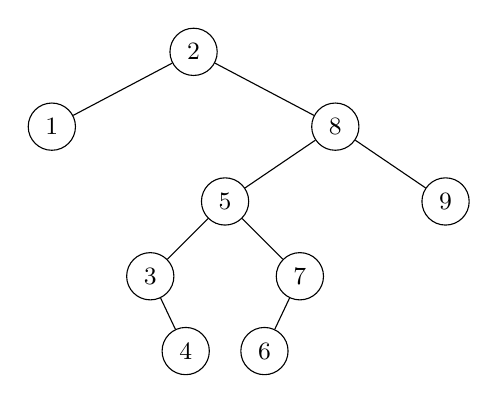
\begin{tikzpicture}[level distance=0.95cm,level 1/.style={sibling distance=3.6cm},
  level 2/.style={sibling distance=2.8cm},level 3/.style={sibling distance=1.9cm},
  level 4/.style={sibling distance=0.9cm},
  every node/.style={circle,draw,minimum size=6mm,inner sep=0pt,font=\small}]
\node {2}
  child {node {1}}
  child {node {8}
    child {node {5}
      child {node {3} child[missing] child {node {4}}}
      child {node {7} child {node {6}} child[missing]}}
    child {node {9}}};
\end{tikzpicture}
\end{center}
三種走訪（資結書第~7.3~節）：
\begin{itemize}
\item 前序：$2, 1, 8, 5, 3, 4, 7, 6, 9$
\item 中序：$1, 2, 3, 4, 5, 6, 7, 8, 9$（二元搜尋樹的中序就是由小到大）
\item 後序：$1, 4, 3, 6, 7, 5, 9, 8, 2$
\end{itemize}

\begin{itemize}
\item (A) 對。 最長的路徑是 $2 \to 8 \to 5 \to 3 \to 4$ 或 $2 \to 8 \to 5 \to 7 \to 6$，$4$ 條邊，葉節點高度 $0$ 的定義下樹高 $4$。
\item (B) 對。 前序中 $8$ 是第 $3$ 個，$3$ 是第 $5$ 個。 （$3$ 在 $8$ 的子樹裡，前序一定先列祖先。）
\item (C) 錯。 後序最後才列根，$2$ 是最後一個，排在 $7$ 後面。
\item (D) 對。 中序由小到大，$4$ 在 $5$ 前面。
\item (E) 錯。 $3$ 的父節點是 $5$，$9$ 的父節點是 $8$，不是兄弟。 $9$ 的兄弟是 $5$，$3$ 的兄弟是 $7$。
\end{itemize}
\end{pastsoln}
